\documentclass[11pt]{article}

\usepackage[utf8]{inputenc}
\usepackage[spanish]{babel}
\usepackage{fullpage}
\usepackage[top=2cm, bottom=4.5cm, left=2.5cm, right=2.5cm]{geometry}
\usepackage{amsmath, amssymb}
\usepackage{enumitem}
\usepackage{fancyhdr}
\usepackage{hyperref}
\usepackage{graphicx}
\usepackage{subcaption}
\usepackage{float}
\usepackage{hyperref}
\usepackage{fancyhdr}
\pagestyle{fancyplain}
\headheight 35pt
\rhead{7 de Diciembre de 2019}
\lhead{Fundamentos de Bases de Datos}
\headsep 1.5em
\newcommand{\setFooterR}[1]{
    \fancyfoot[R]{\small\textit{#1}}
}

\fancyfoot[C]{}
\renewcommand{\footrulewidth}{0.4pt}
\setFooterR{\href{}{TaqueroMucho.com}}
\begin{document}

\begin{center}
	\LARGE{\textbf{Proyecto Final\\Reporte de Resultados\\TaqueroMucho}}
\end{center}

\section{Consultas propuestas }
\subsection{Sucursal que más ha vendido.}
\includegraphics[width=8cm]{un.png}
\subsection{Ganancia por dia en sucursales.}
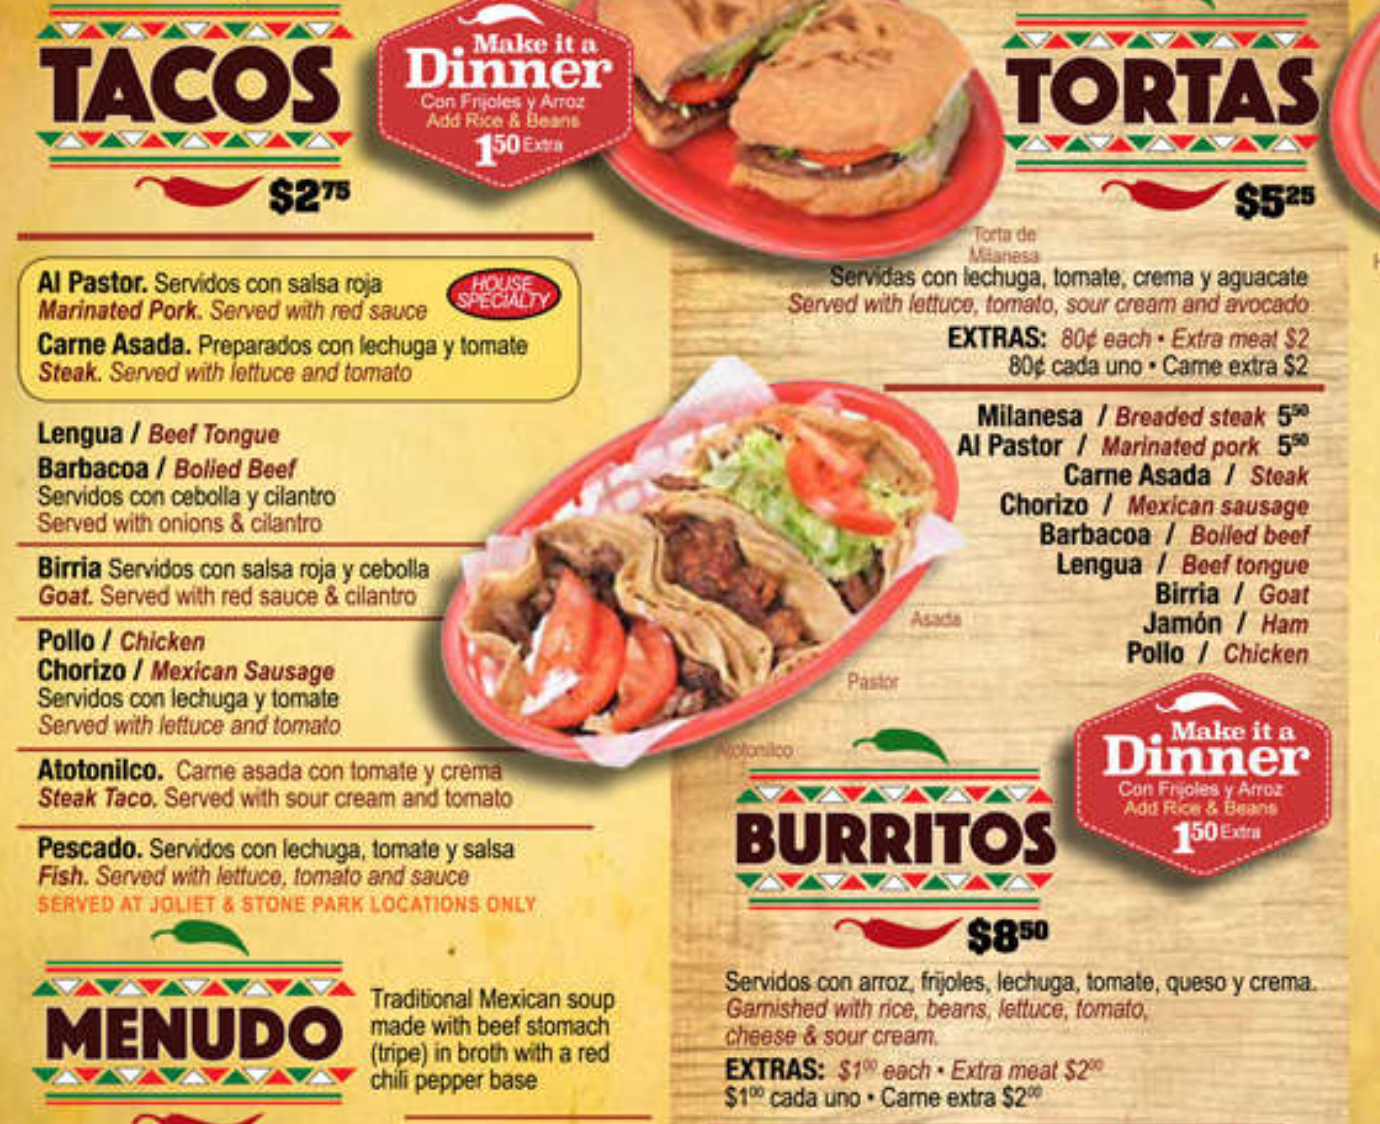
\includegraphics[width=8cm]{dos.png}
\subsection{Tiempo que lleva cada empleado en las sucursales que ha trabajado.}
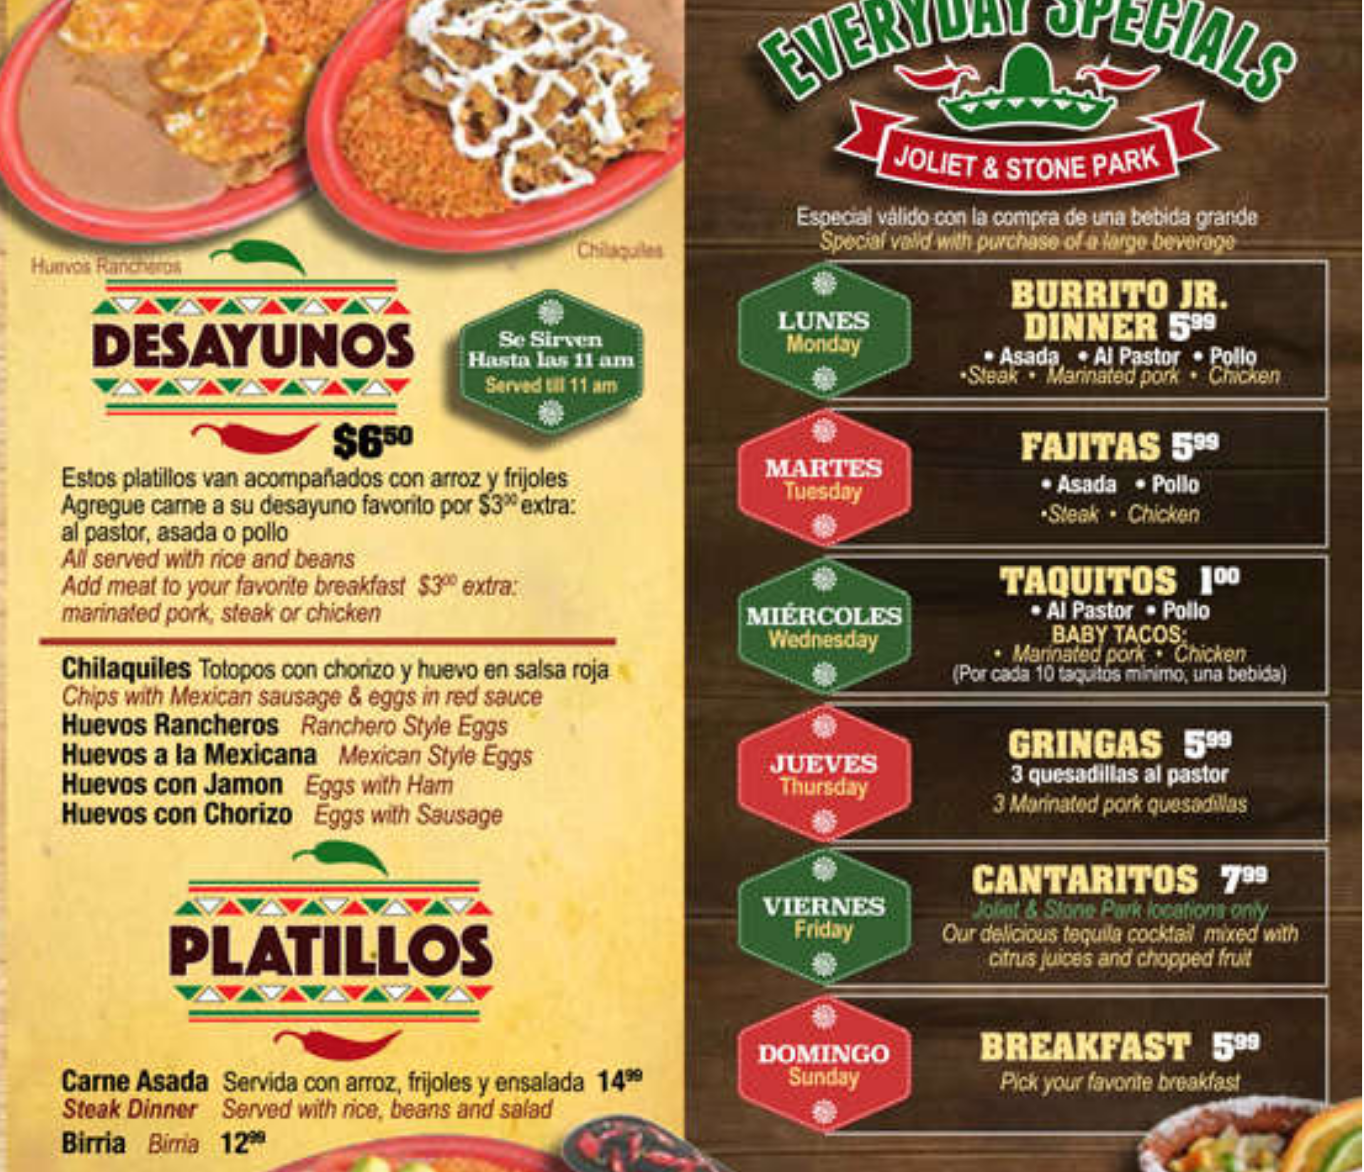
\includegraphics[width=8cm]{tres.png}
\subsection{Ventas totales de cada platillo.}
\includegraphics[width=8cm]{4.png}
\subsection{El proveedor al que más se le compra.}
\includegraphics[width=8cm]{5.png}
\subsection{Precio actual de cada platillo por sucursal.}
\includegraphics[width=8cm]{6.png}
\subsection{Platillos más vendidos usando efectivo.}
\includegraphics[width=8cm]{7.png}
\subsection{Numero de platillo entregados por tipo de transporte en cada sucursal.}
\includegraphics[width=8cm]{8.png}
\subsection{Numero de clientes del estado con mas usuarios.}
\includegraphics[width=8cm]{9.png}
\subsection{ Veces que cada metodo de pago ha sido usado en cada sucursal.}
\includegraphics[width=8cm]{10.png}
\subsection{Los platillos que lleven más de 4 ingredientes y cuesten mas de 60 pesos.}
\includegraphics[width=8cm]{11.png}
\subsection{El total de todos los pagos hechos a empleados.}
\includegraphics[width=8cm]{12.png}
\subsection{La cantidad de dinero que más ha gastado un cliente en los últimos 6 meses en cada sucursal.}
\includegraphics[width=8cm]{13.png}
\subsection{La salsa más vendida junto con tacos.}
\includegraphics[width=8cm]{14.png}
\subsection{El tipo de ingrediente más utilizado en tacos.}
\includegraphics[width=8cm]{15.png}

\end{document}
